\documentclass{beamer}
\nonstopmode
\usetheme{Boadilla}
%\usetheme{Madrid}
%\usetheme{Pittsburgh}
%\usetheme{Rochester}
\usecolortheme{beaver}
\usecolortheme{orchid}
\setbeameroption{show notes}
\hypersetup{pdfstartview={Fit}} % fits the presentation to the window when first displayed
\usepackage{xcolor}
\usepackage{adjustbox} %Used to fit tables to slides

\usepackage{array} %used for math mode in table aod
\usepackage{import} % \subimput alows importing of Inkscape pdf+tex files in subfolder

\title[Perception and Working Memory in Neglect]{Perceptual and Working Memory Deficits in Unilateral Neglect}
\subtitle{}

\author{Jason Locklin}
\institute[University of Waterloo]
{Department of Psychology\\
	University of Waterloo\\
	\bigskip
	Supervisor: Dr.\ James Danckert
}
\date[August 6, 2015]
{}% <- QR

%\AtBeginSection[]
%{\begin{frame}
%		\frametitle{Experiments}
%		\tableofcontents[currentsection]
%	\end{frame}
%}


\begin{document}

%%%%%%%%%%%%%%%%%%%%%%%% GENERAL INTRODUCTION
\frame{\titlepage}
\section*{}

\begin{frame}
	\frametitle{Unilateral Neglect}
	\begin{columns}
		\begin{column}{0.5\textwidth}
\begin{itemize}
	\item Typically results from damage to the right inferior parietal or superior temporal cortex.
	\bigskip
	\item Inability to respond to the left side of space.
	\end{itemize}
		\end{column}
		\begin{column}{0.5\textwidth}
			\only<1>{ 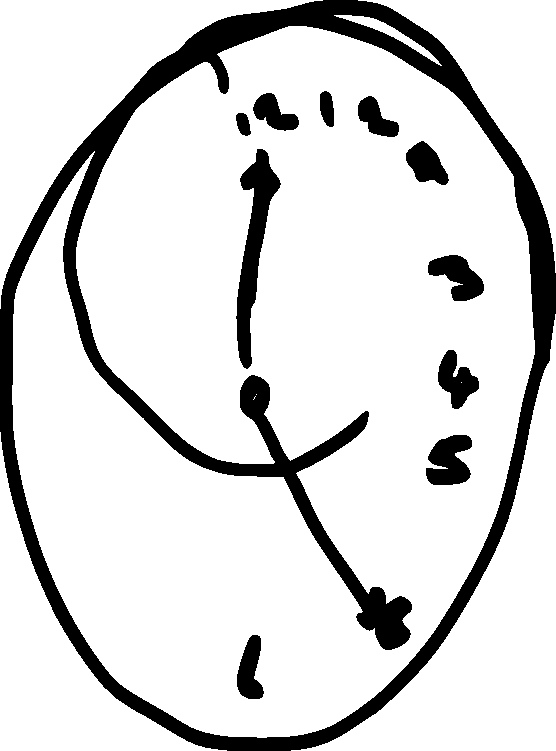
\includegraphics
			[height=.5\textheight,width=\textwidth,keepaspectratio]
			{img/Clock_drawing.pdf}}
			\only<2>{ 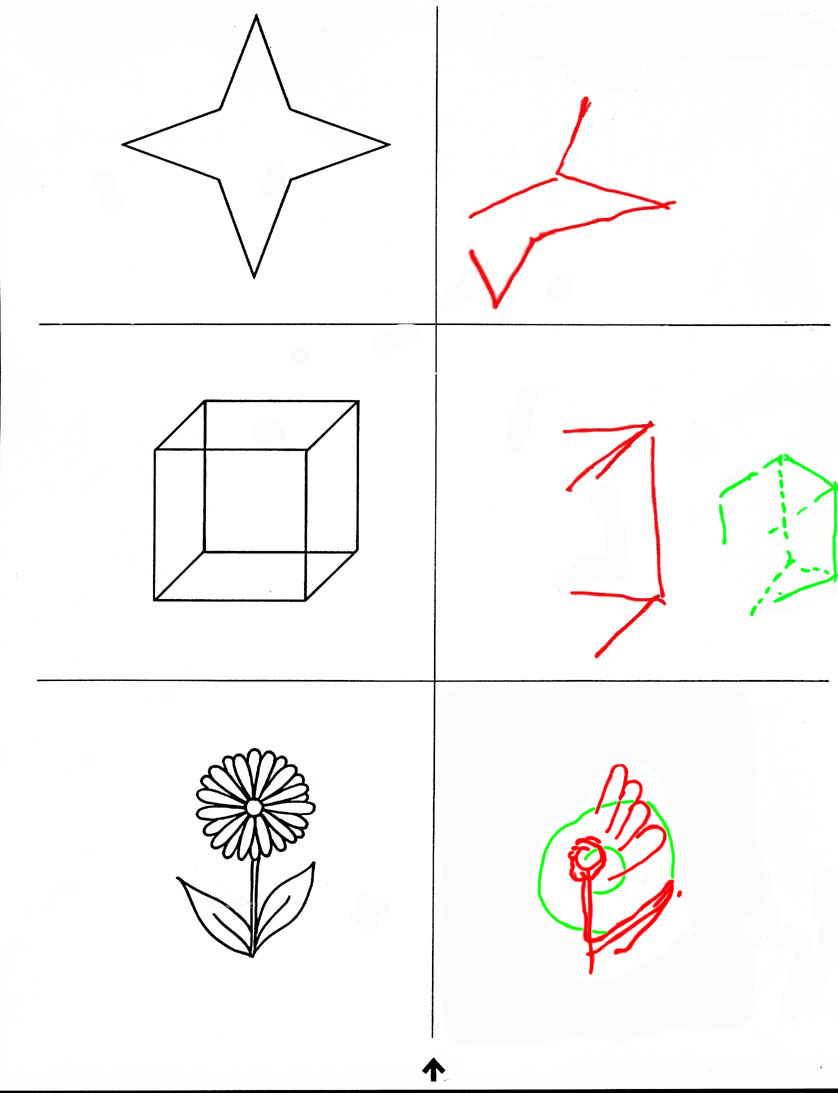
\includegraphics
			[height=.5\textheight,width=\textwidth,keepaspectratio]
			{img/figure_copy.jpg}}
			\only<3>{ 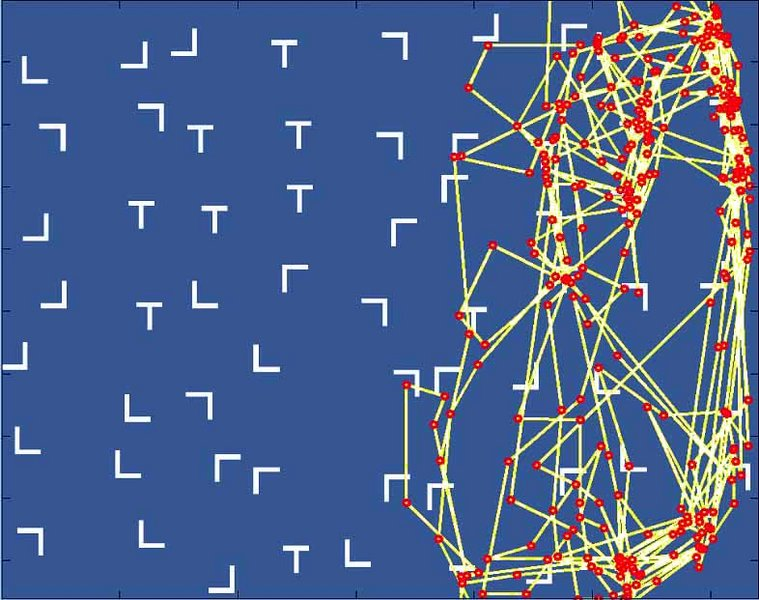
\includegraphics
			[height=.5\textheight,width=\textwidth,keepaspectratio]
			{img/Visual_Search.jpg}}
		\end{column}
	\end{columns}
\end{frame}


\begin{frame}
	\frametitle{Neglect as a Lateralized Dissorder of Attention}
	\begin{columns}
		\begin{column}{0.5\textwidth}
			\begin{itemize}
				\item	Prefferential orienting rightward
				\bigskip
				\item Delayed re-orienting leftward.
				%\item Evidence from covert orienting and visual search.
				%\item Other non-lateralized deficits of attention such as selective attention (attentional blink), and sustained attention.
			\end{itemize}
		\end{column}
		\begin{column}{0.5\textwidth}
			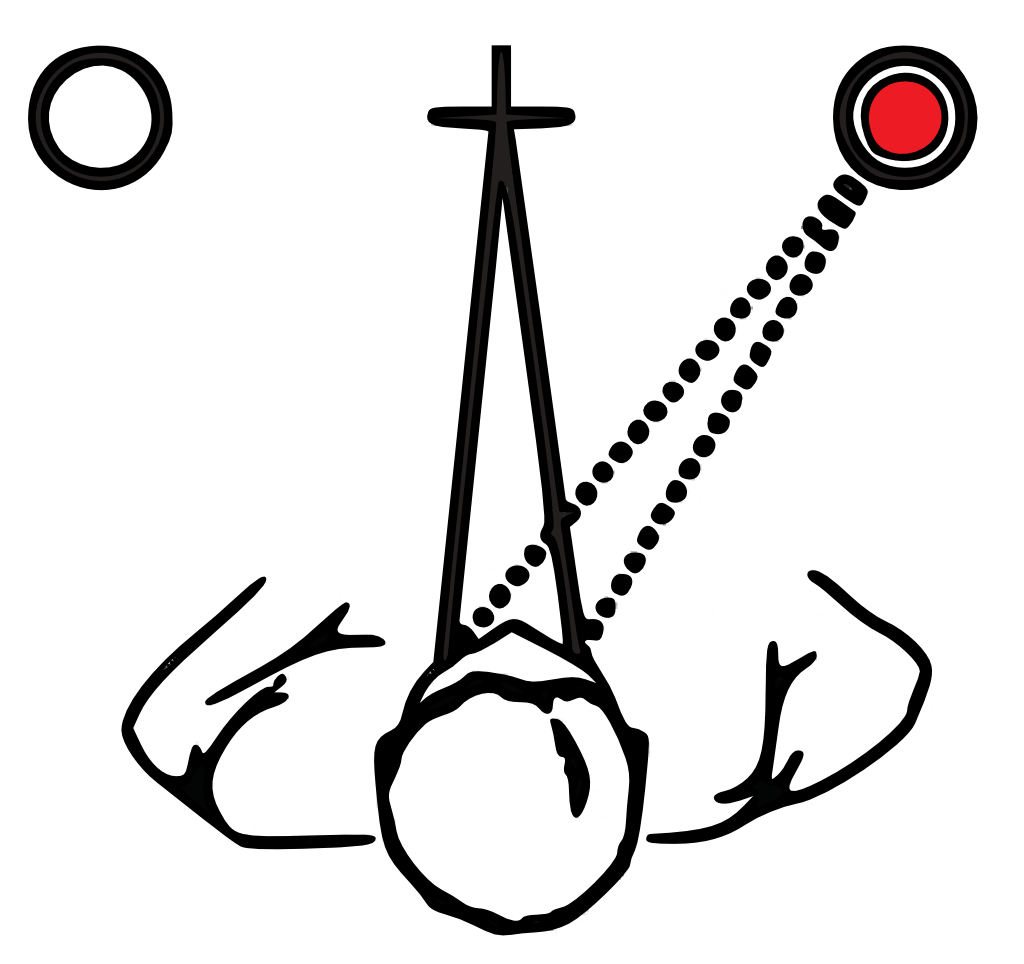
\includegraphics
			[height=.5\textheight,width=\textwidth,keepaspectratio]
			{img/orienting.png}
		\end{column}
	\end{columns}
	\end{frame}


\begin{frame}
	\frametitle{Impaired Perceptual Representation as a Key Component of Neglect}
	\begin{block}{Perceptual deficits:}
		\begin{itemize}
			\item Chimeric face perception
			\item Perceptual judgement of spatial extent.
		\end{itemize}
	\end{block}
	\begin{block}{Working Memory deficits:}
		\begin{itemize}
		\item Spatial Working Memory.
		\end{itemize}
	\end{block}
\end{frame}

\begin{frame}
	\frametitle{Spatial Working Memory}
	\centering 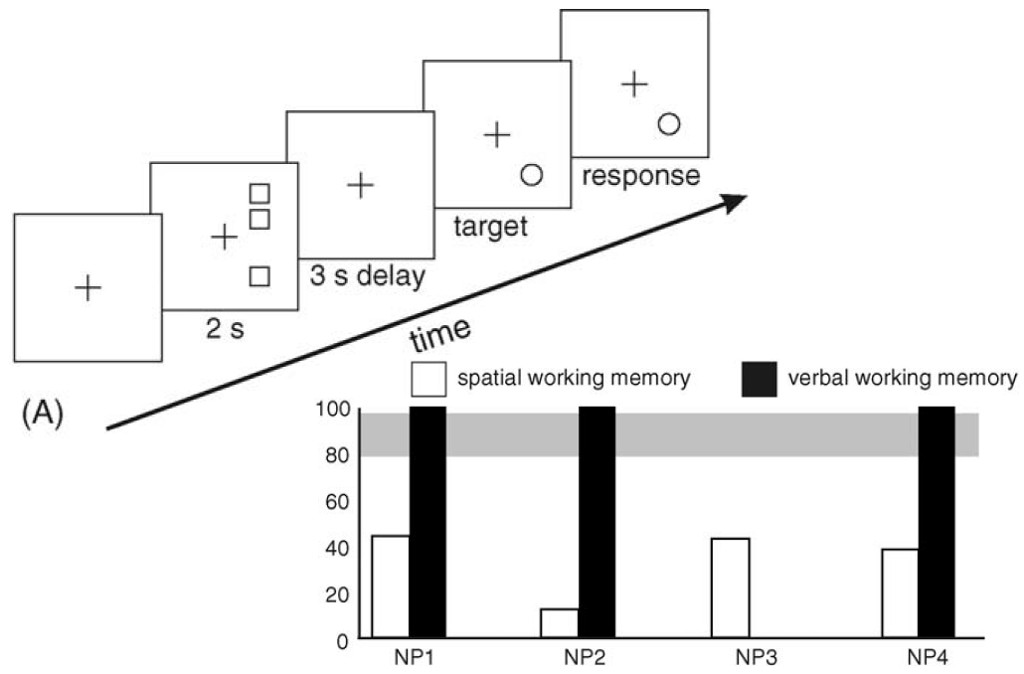
\includegraphics
			[height=.8\textheight,keepaspectratio]
			{img/danckert2006.png}\\
	\tiny (Danckert \& Ferber 2006)
\end{frame}

\begin{frame}
	\frametitle{Possible Explenations of Observed Working Memory (WM) deficits}
	\begin{enumerate}
		\item WM intact, but WM tasks influenced by attention deficits.
		\item WM intact, but degraded when it needs access to spatial attention for rehursal.
		\item WM impaired by neglect-inducing parietal lesion
	\end{enumerate}
\end{frame}

% fade the first as implausible given the evidence
\begin{frame}
	\frametitle{Possible Explenations of Observed Working Memory (WM) deficits}
	\begin{enumerate}
		\item \textcolor{gray}{WM intact, but WM tasks influenced by attention deficits.}
		\item WM intact, but degraded where it would normally accesses spatial attention for rehursal.
		\item WM impaired by neglect-inducing lesion.
	\end{enumerate}
\end{frame}

%%%%%%%%%%%%%%%%%%%%%%% EXPERIMENT ONE

\section[Attention and WM]{Examine non-spatial ``visual'' WM and compare with attention}

\begin{frame}
	\frametitle{Experiment 1: WM deficits or Rehursal Failure?}
		\tableofcontents[currentsection]
\end{frame}

\begin{frame}
\frametitle{Participants}

\end{frame}

%%%% VWM
\subsection*{Visual Working Memory}

\begin{frame}
	\frametitle{Visual Working Memory Task}
	\def\svgwidth{\textwidth}
	\subimport{VWM/}{VWM/fig_VWM-task.pdf_tex}
\end{frame}

\begin{frame}
	\frametitle{Response Model Calculations}
	To be added: Slides to explain prob. models based off Fig 2.2.\\
	Need to figure out the best way to explain this fluidly, and also a more thorough
	explenation using appendix slidess if necissary.
\end{frame}

\begin{frame}
	\frametitle{Figure 2.3}
	\centering
	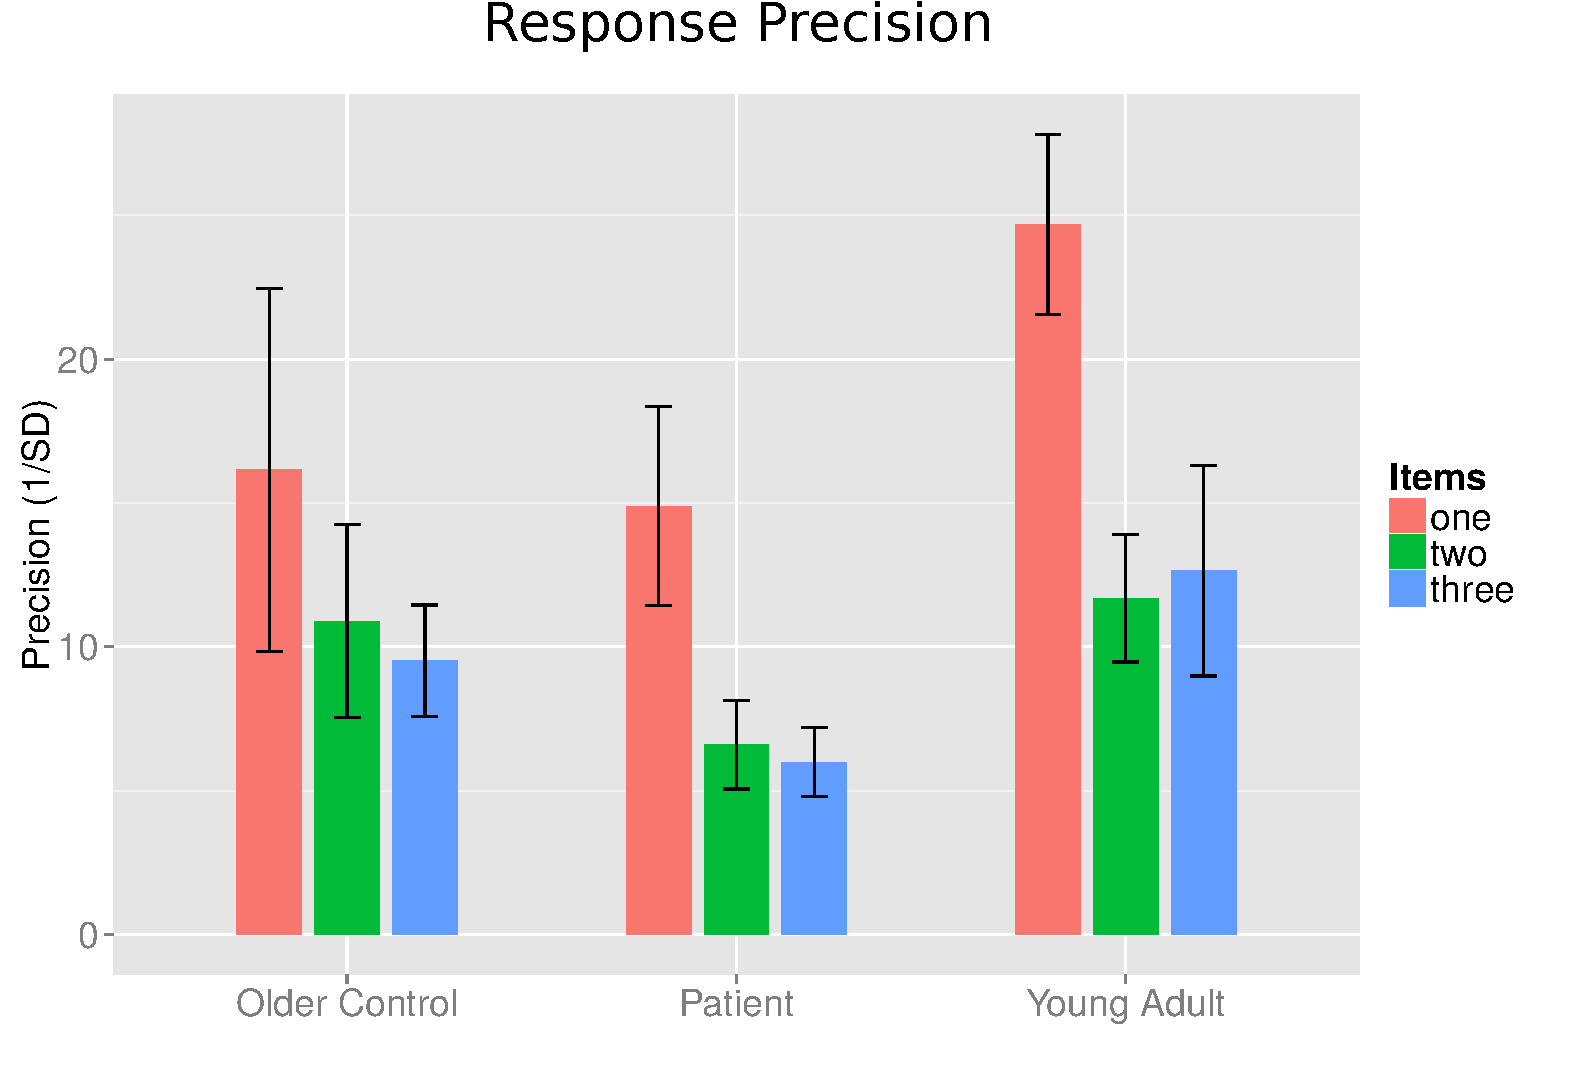
\includegraphics
	[height=.8\textheight,width=\textwidth,keepaspectratio]
	{VWM/fig_VWM_Precision.pdf}
\end{frame}

\begin{frame}
	\frametitle{Figure 2.4}
	\centering
	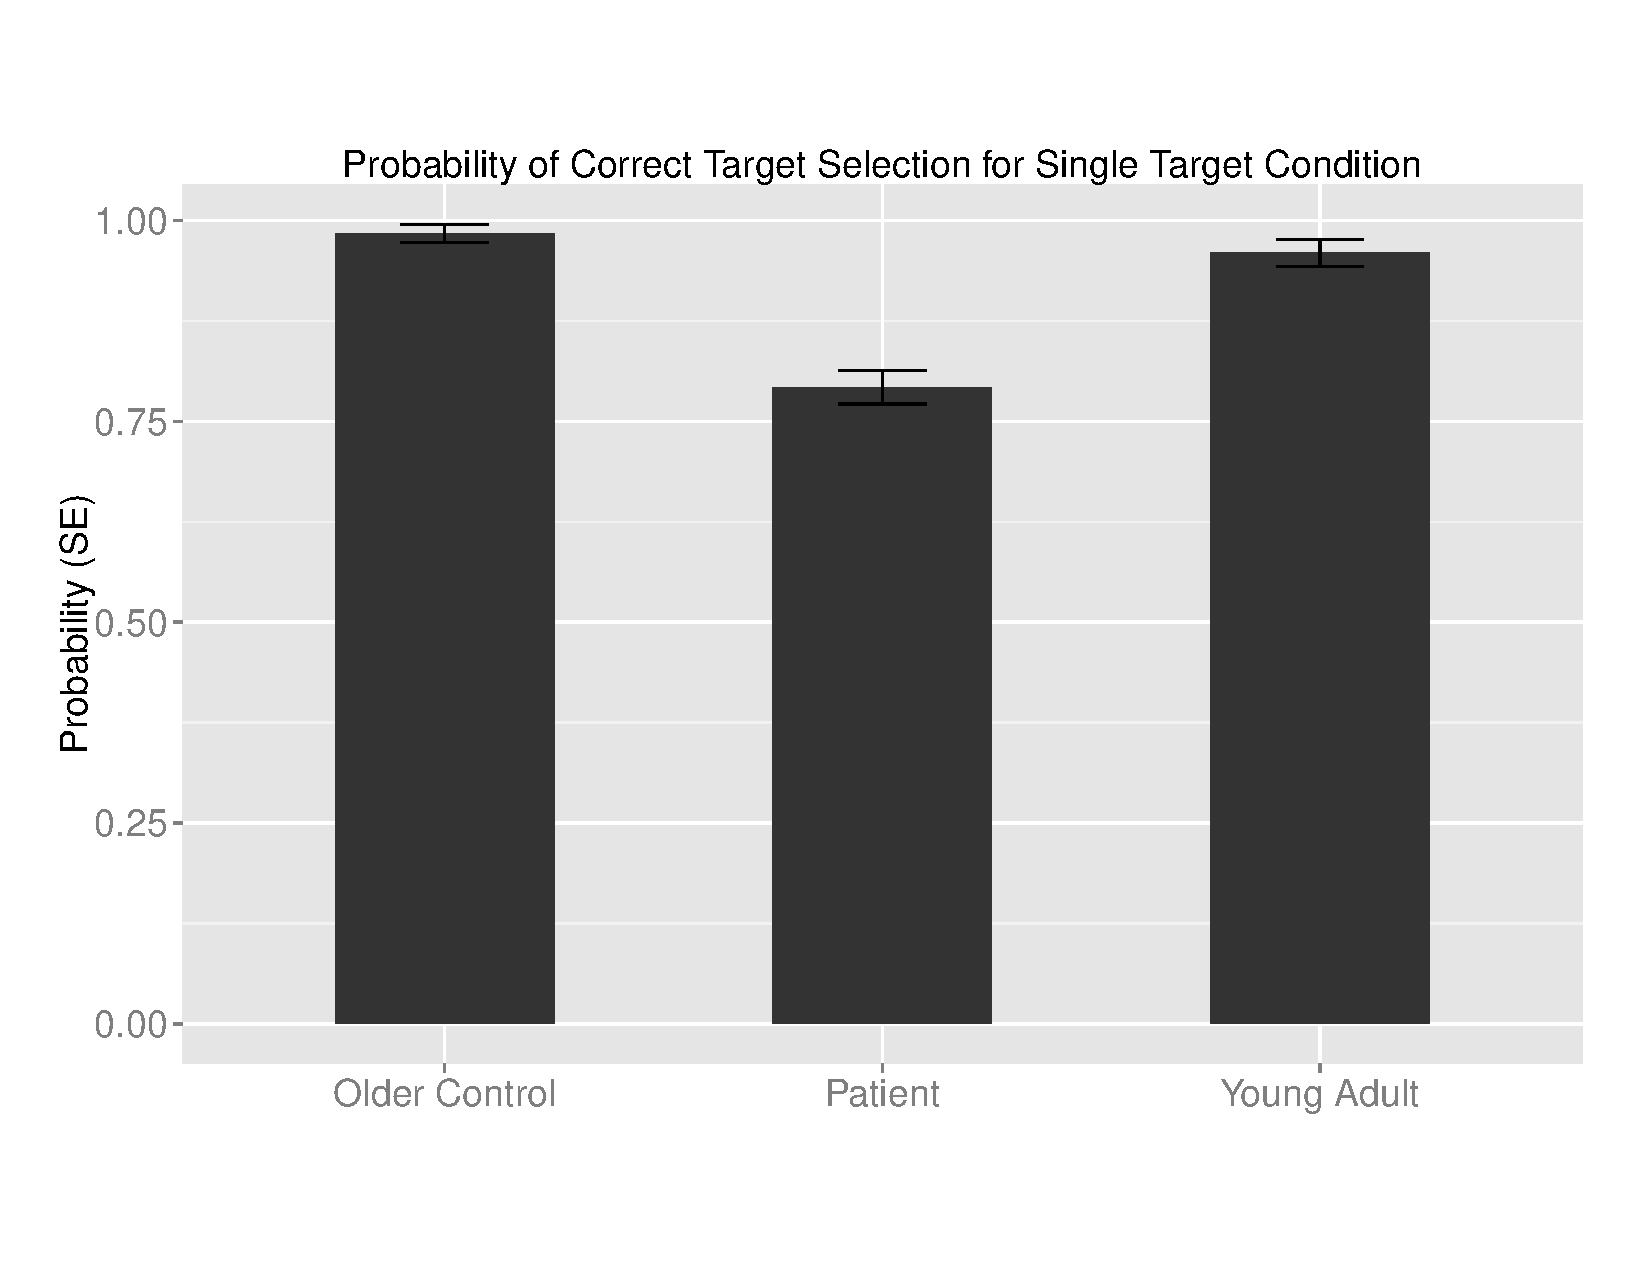
\includegraphics
	[height=.8\textheight,width=\textwidth,keepaspectratio]
	{VWM/fig_VWM_1Target.pdf}
\end{frame}

\begin{frame}
	\frametitle{Figure 2.5}
	\centering
	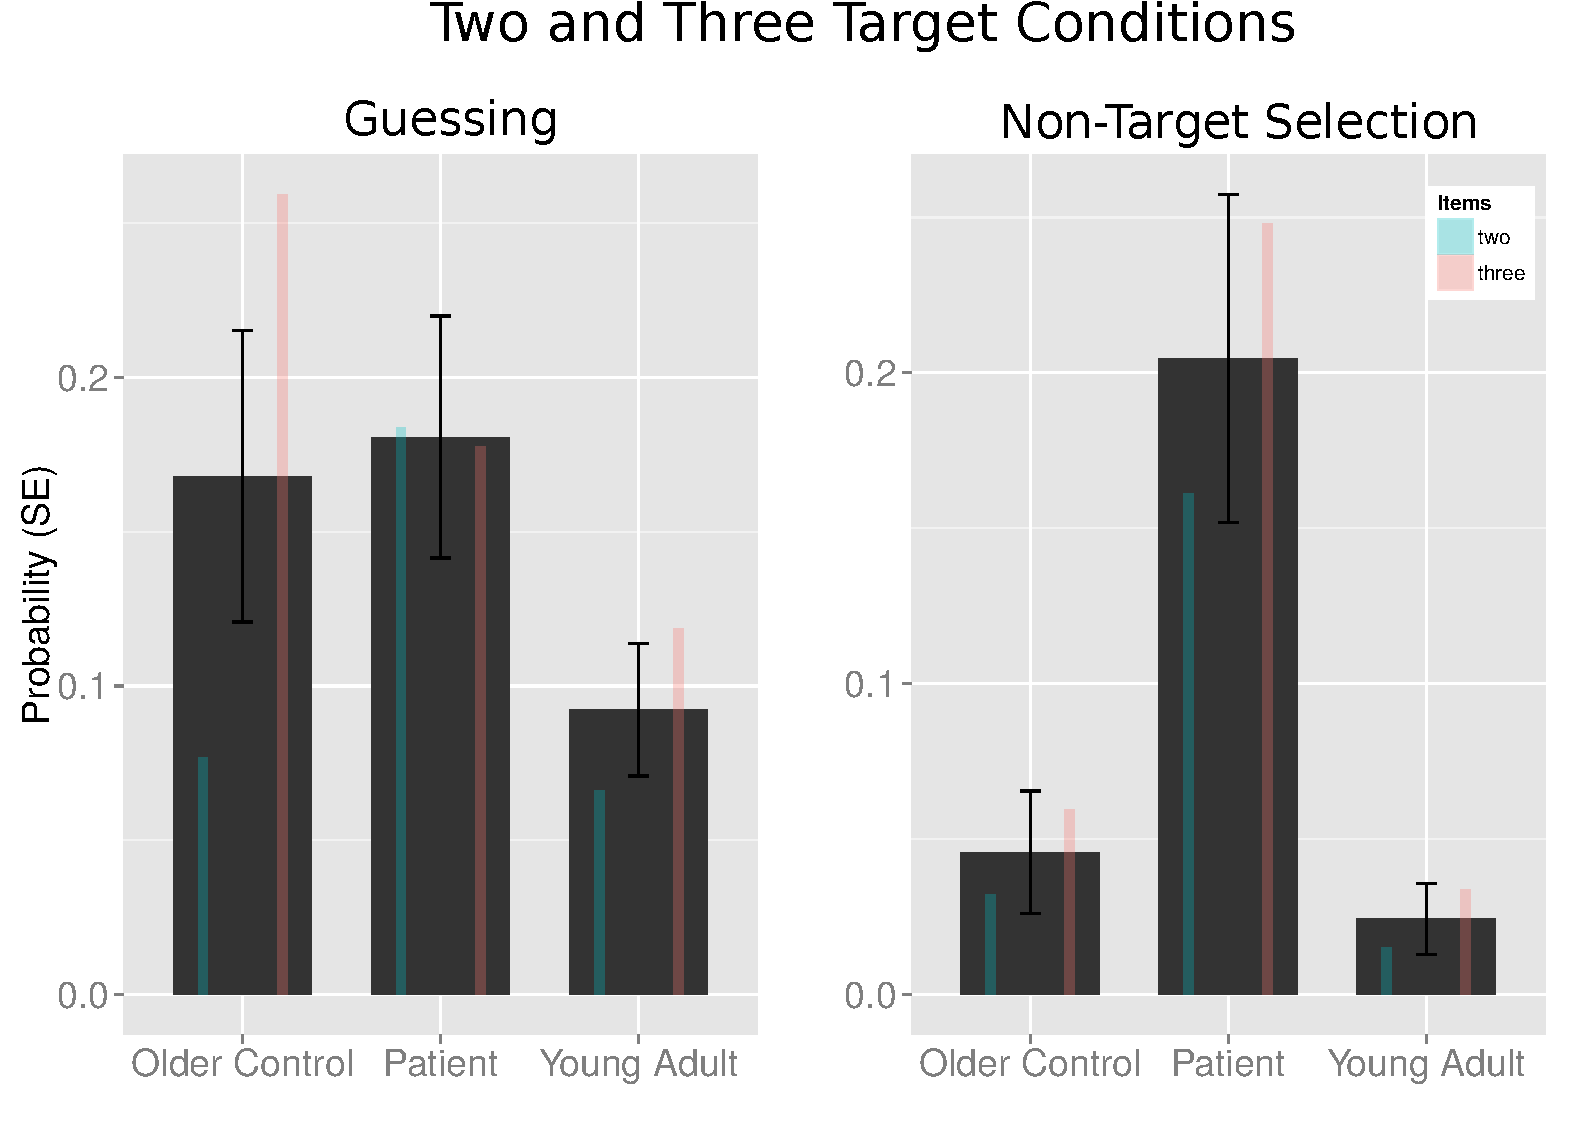
\includegraphics
	[height=.8\textheight,width=\textwidth,keepaspectratio]
	{VWM/fig_VWM_MTarget.pdf}
\end{frame}


%%%% COVAT
\subsection*{Covert Orienting}
\begin{frame}
	\frametitle{Covert Orienting Task}
	\def\svgwidth{\textwidth}
	\subimport{VWM/}{VWM/fig_COVAT-task.pdf_tex}
\end{frame}

\begin{frame}
	\frametitle{Figure 2.6}
	\centering
	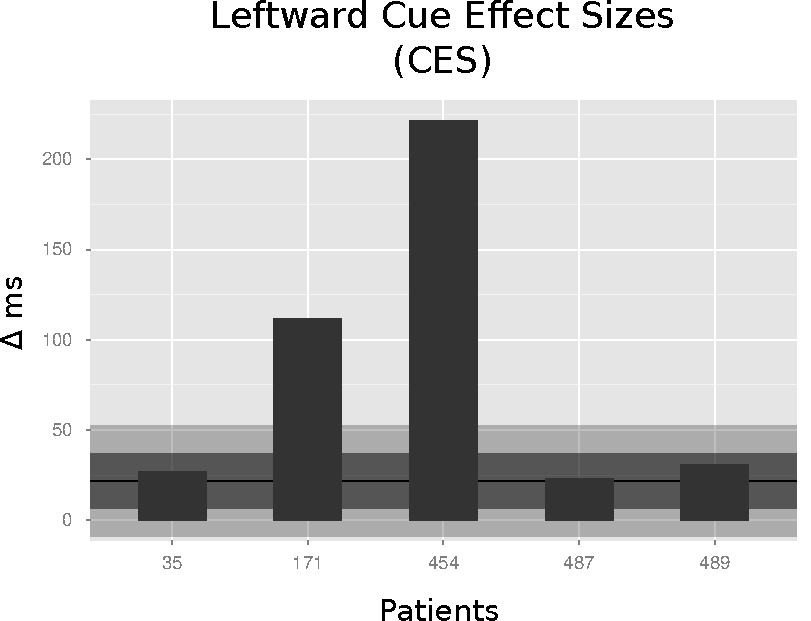
\includegraphics
	[height=.8\textheight,width=\textwidth,keepaspectratio]
	{VWM/fig_COVAT.pdf}
\end{frame}

\subsection*{}
\begin{frame}
	\frametitle{Comparison}
	to be added: slide(s) illustrating the comparison of the two tasks
\end{frame}

\begin{frame}
	\frametitle{Recovery of Attention and Perceptual Representations}
	If deficits of perceptual representation in neglect are independant of spatial attention deficits,
	then treatment of spatial attention deficits will not improve perceptual representation
\end{frame}

\begin{frame}
	\frametitle{Prism Adaptation}
	Basic prism adaptation description
\end{frame}

\begin{frame}
	\frametitle{Prism Adaptation Improves of (re)orienting, but Produces Limited Change in Perceptual Awareness}
	\begin{itemize}
		\item Prisms improve leftward re-orienting
		\item Perception of spatial extent and chimeric faces provide evidence of limited change in awareness.
	\end{itemize}
\end{frame}

%%%%%%%%%%%%%%%%%%%%%%%% EXPERIMENT TWO
\section[Prisms]{Prism Adaptation and Perceptual Representation}

\begin{frame}
	\frametitle{Experiment 2: Does treatment of attention deficits influence perceptual representations?}
		\tableofcontents[currentsection]
\end{frame}


\begin{frame}
	\frametitle{Participants}
\begin{itemize}
	\item 
\end{itemize}
\end{frame}

\begin{frame}
	\frametitle{Figure 3.4}
	\centering
	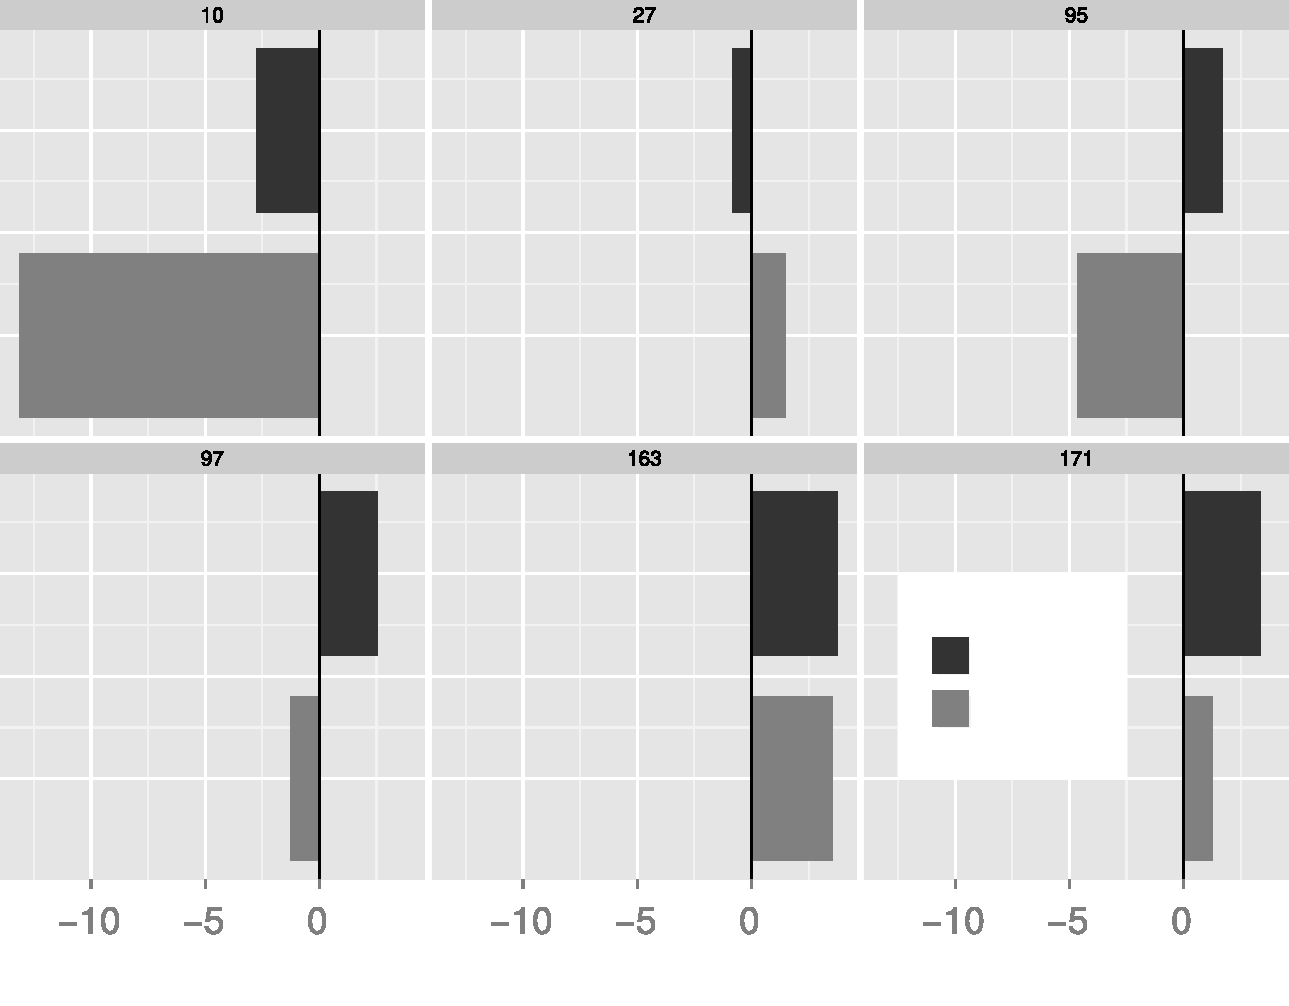
\includegraphics
	[height=.85\textheight,width=\textwidth,keepaspectratio]
	{Prisms/fig_LB_Prisms.pdf}
\end{frame}


%%%% SWM
\subsection*{Spatial Working Memory}

\begin{frame}
	\frametitle{Spatial Working Memory Task}
	\def\svgwidth{0.7\textwidth}
	\subimport{Prisms/}{Prisms/fig_SWM-task.pdf_tex}
\end{frame}

\begin{frame}
	\frametitle{Figure 3.2}
	\centering
	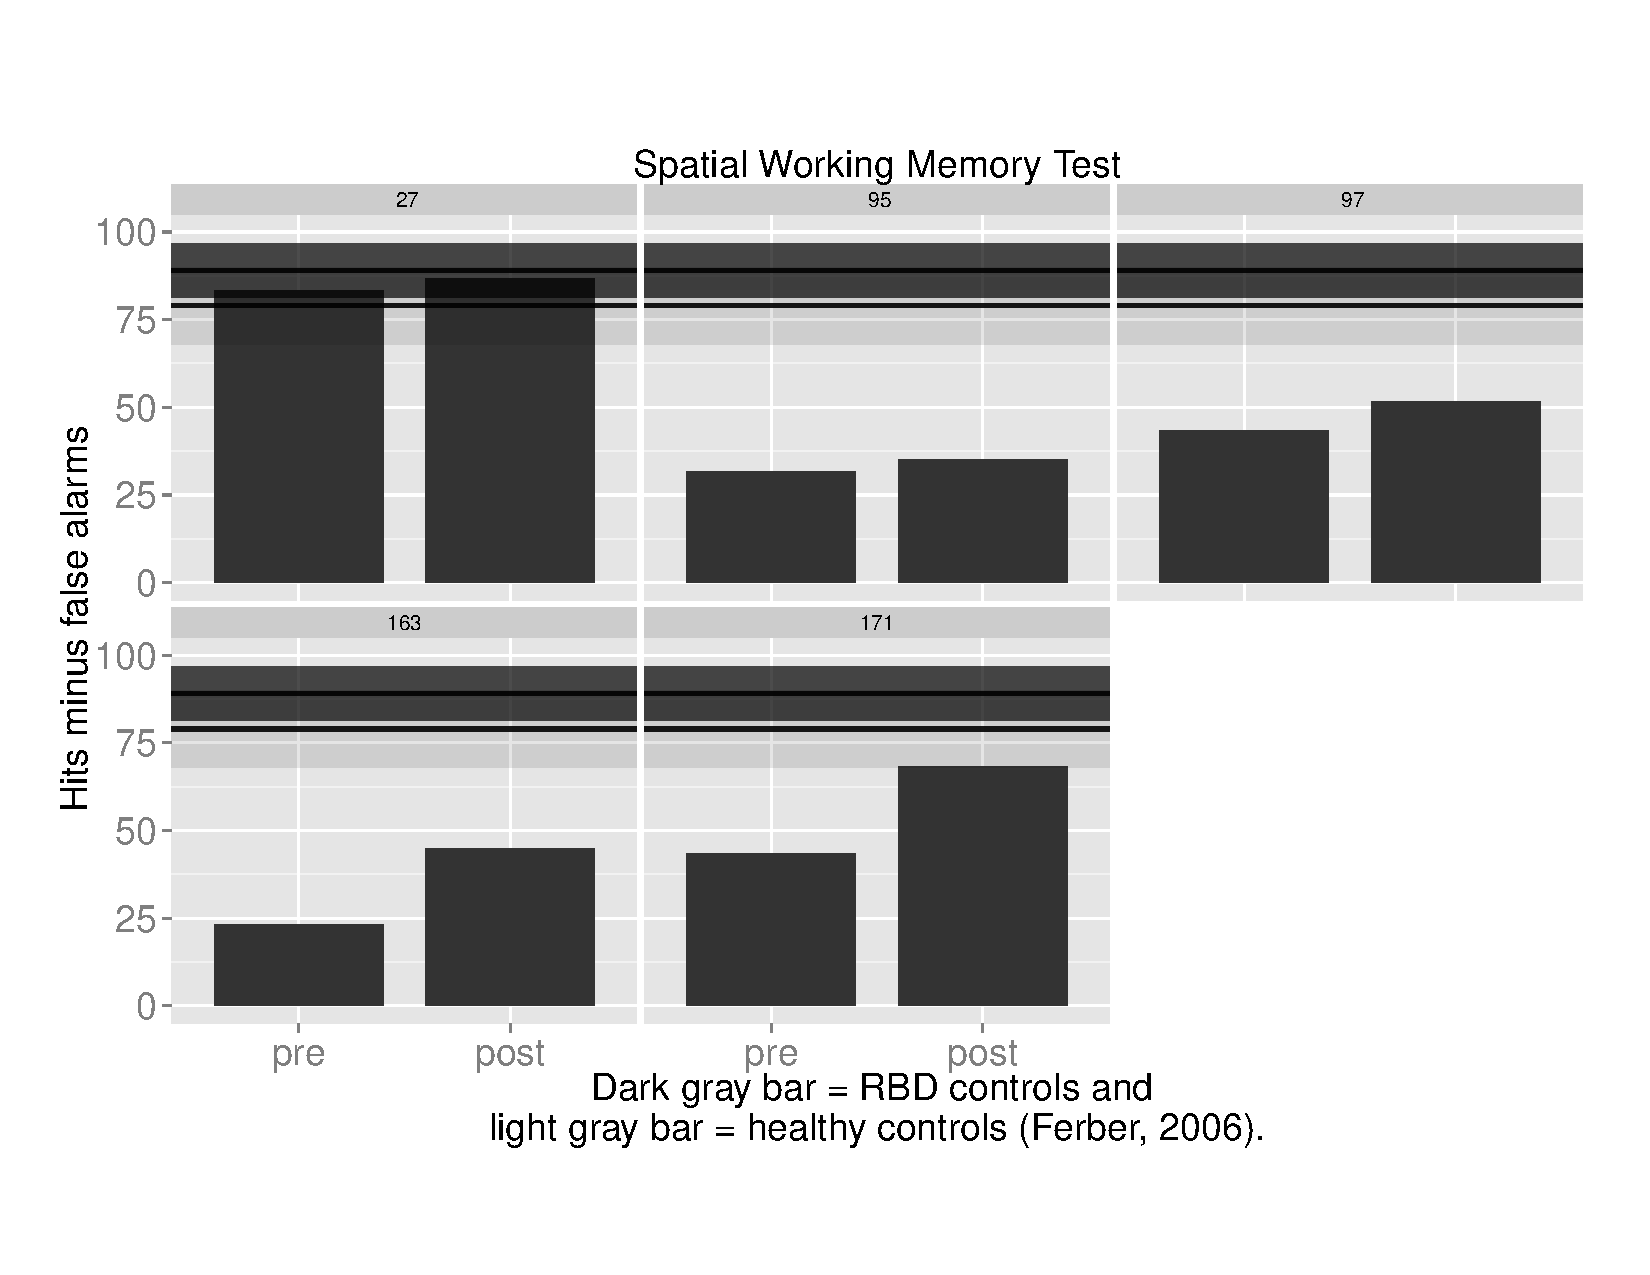
\includegraphics
	[height=.85\textheight,width=\textwidth,keepaspectratio]
	{Prisms/fig_SWM.pdf}
\end{frame}


%%%% TE
\subsection*{Time Perception}
\begin{frame}
	\frametitle{Temporal Estimation Task}
	\def\svgwidth{0.9\textwidth}
	\subimport{Prisms/}{Prisms/fig_TE-task.pdf_tex}
\end{frame}

\begin{frame}
	\frametitle{Figure 3.3}
	\centering
	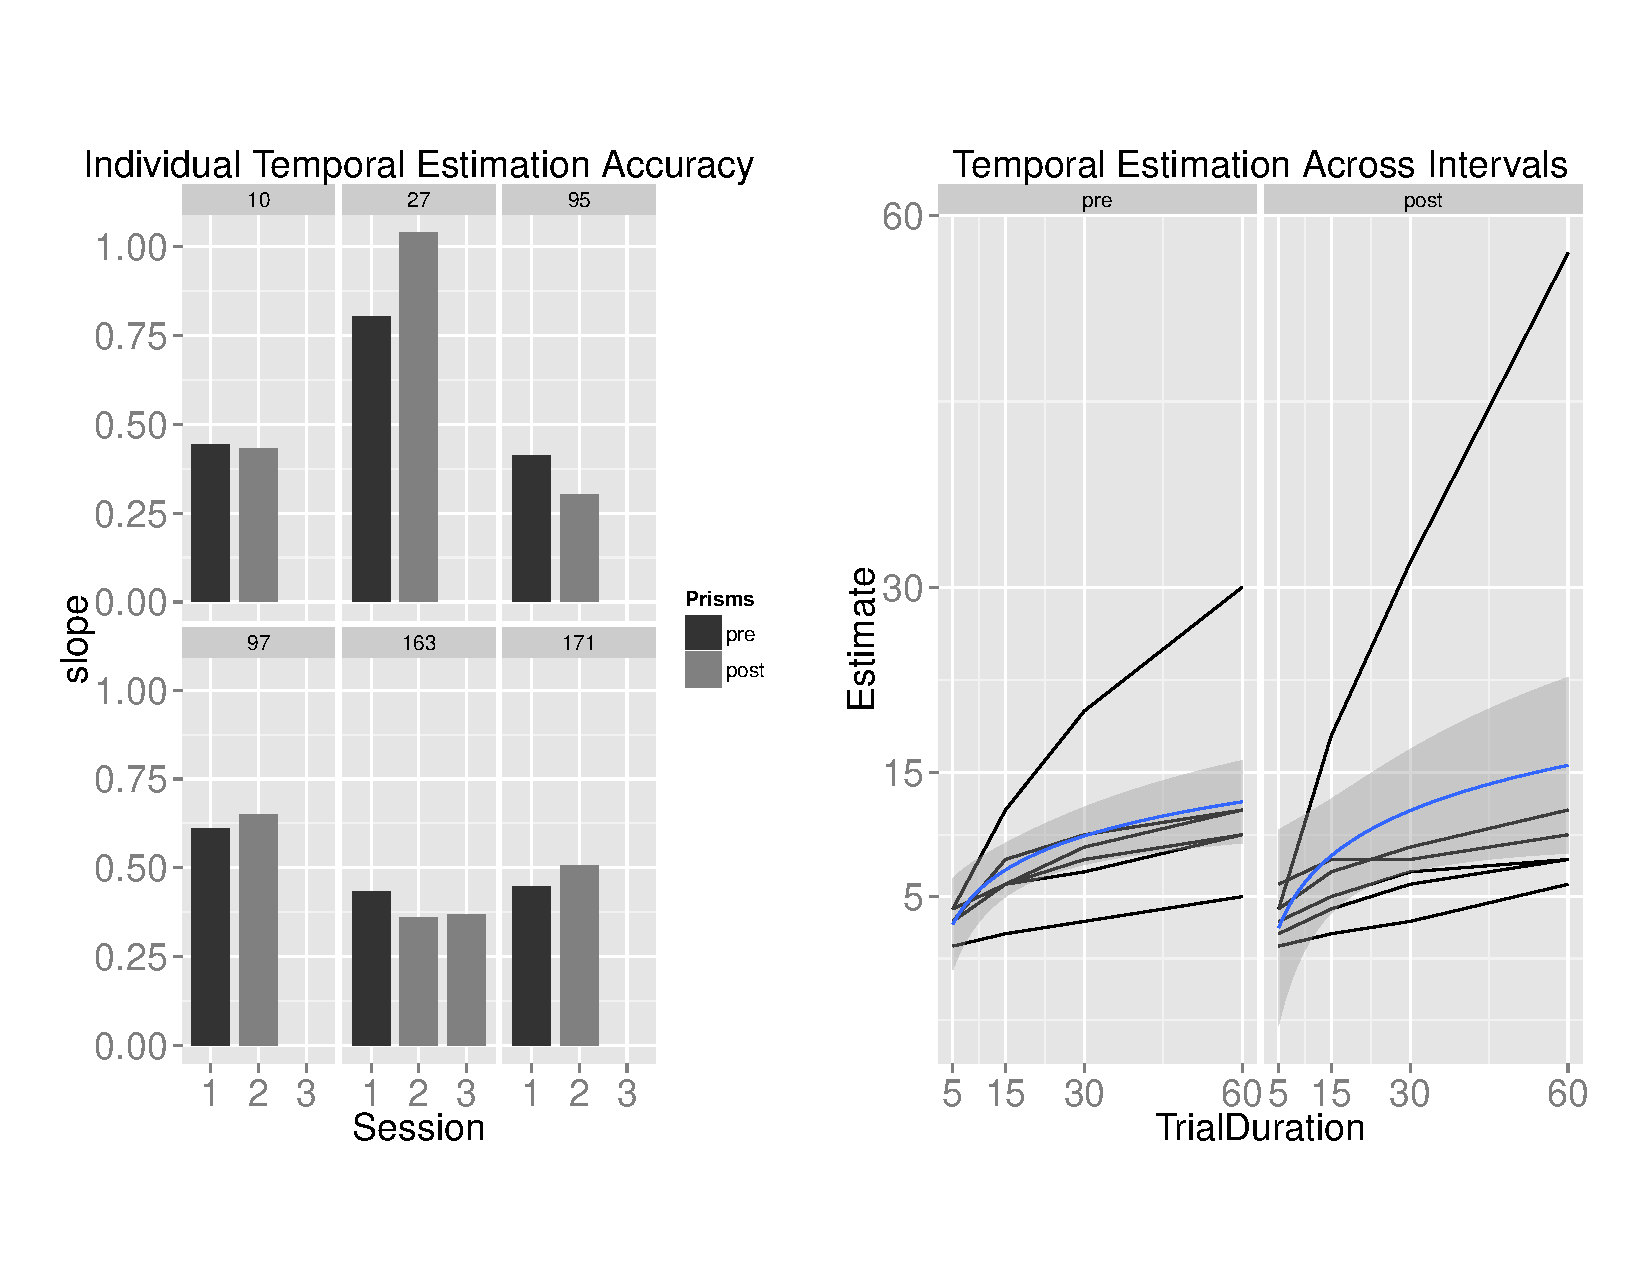
\includegraphics
	[height=.75\textheight,width=\textwidth,keepaspectratio]
	{Prisms/fig_TE.pdf}
\end{frame}



\subsection*{}
\begin{frame}
	\frametitle{Prisms are not influencing perceptual representations, \\ so what will?}
	Saccadic adaptation is simmilar to prism adaptation, but produces subtle effects on perception.
	\begin{itemize}
		\item Example
		\item example
	\end{itemize}
\end{frame}


%%%%%%%%%%%%%%%%%%%%%%%% EXPERIMENT THREE
\section[Saccadic Adaptation]{Saccadic Adaptation for Action and Perception}

\begin{frame}
	\frametitle{Experiment 3: Does Saccadic Adaptation influence perceptual representations?}
		\tableofcontents[currentsection]
\end{frame}

\begin{frame}
	\frametitle{Landmark and Line Bisection Tasks}
	Striemer \& Danckert 2010a
\end{frame}

\begin{frame}
	\frametitle{Landmark Task}
	\def\svgwidth{0.8\textwidth}
	\subimport{SA/}{SA/fig_Landmark-task.pdf_tex}
\end{frame}


\begin{frame}logic shorthand causal relationship
	\frametitle{Line Bisection Task}
	\def\svgwidth{0.9\textwidth}
	\subimport{SA/}{SA/fig_LineBisection.pdf_tex}
\end{frame}

\begin{frame}
	\frametitle{Saccadic Adaptation}
	\centering
	\def\svgwidth{0.7\textwidth}
	\tiny
	\subimport{SA/}{SA/fig_SA.pdf_tex}
\end{frame}


\begin{frame}
	\frametitle{Analysis of an Example Saccade}
	\centering
	\def\svgwidth{\textwidth}
	\tiny
	\subimport{SA/}{SA/fig_Saccade.pdf_tex}
\end{frame}

\begin{frame}
	\frametitle{Figure 3.3: Effect of Saccadic Adaptation}
	\centering
	\def\svgwidth{0.9\textwidth}
	\tiny
	\subimport{SA/}{SA/fig_Adaptation.pdf_tex}
\end{frame}

\begin{frame}
	\frametitle{Impact on Line Bisection (LB) and Landmark Task (LT)}
	Figure TBD.
\end{frame}


%%%%%%%%%%%%%%%%%%%%%%%% CONCLUDING MATTER
\section*{}
\begin{frame}
	\frametitle{Conclusions}
	text goes here
\end{frame}

\begin{frame}
	\frametitle{Future Directions}
	\begin{itemize}
		\item Improve SA procedure, possibly with whole-field Adaptation
		\item Increase duration of Prism Adaptation and utilize terminal rather than concurrent feedback.
		\item If successfull, compare the two in a neglect population.
	\end{itemize}
\end{frame}

\begin{frame}
	\frametitle{Awknowledgements}
	Supervisor: Dr. James Danckert
	DAAG lab, funding agencies, etc.
\end{frame}


%%%%%%%%%%%%%%%%%%%%%%%% APPENDIX
\subsection*{Appendix}
\begin{frame}[noframenumbering]
	\frametitle{Table 2.1}
	\adjustbox{max height=\dimexpr\textheight-5.5cm\relax,
	max width=\textwidth}{\begin{tabular}{rrllrrrrlr}
  \hline
 & Age & Sex & Handedness & CES & VWM(1) & VWM(2/3) & Stars & Copying & Bisection \\ 
  \hline
487 &  61 & F & Right & 23.0 & 0.15 & 0.04 & 0& + & 2.2 \\ 
  35 &  51 & F & Right & 27.0 & 0.15 & 0.04 & 17& + & 0.1 \\ 
  489 &  66 & M & Left & 31.0 & 0.25 & 0.08 & 0& + & 1.0 \\ 
  171 &  71 & F & Left & 112.0 & 0.13 & 0.00 & 0& -  & 1.4 \\ 
  454 &  70 & M & Right & 221.5 & 0.23 & 0.17 & 0& + & 6.3 \\ 
  213 &  65 & F & Right & NA & 0.2 & 0.30 & 100& + & 7.3 \\ 
  396 &  85 & M & Right & NA & 0.3 & 0.55 & 87& + & 8.1 \\ 
  465 &  63 & F & Right & NA & 0.3 & 0.45 & 97& + & 12.9 \\ 
   \hline
\end{tabular}
}
\end{frame}

\begin{frame}[noframenumbering]
	\frametitle{Table 2.2}
	% latex table generated in R 3.1.1 by xtable 1.7-4 package
% Wed Apr 15 20:12:57 2015
\begin{table}[ht]
\centering
\begin{tabular}{lrrrrr}
  \hline
 & Df & Deviance & Resid. Df & Resid. Dev & Pr($>$Chi) \\ 
  \hline
NULL &  &  & 15 & 22.18 &  \\ 
  CES & 1 & 8.62 & 14 & 13.56 & 0.0033 \\ 
  $P_{NT}$ & 1 & 1.12 & 13 & 12.44 & 0.2908 \\ 
  $P_G$ & 1 & 12.44 & 12 & 0.00 & 0.0004 \\ 
   \hline
\end{tabular}
\caption{Analysis of deviance table. Each row represents the change in
	deviance of the model with the addition of one term. Pr($>$Chi) is the
	probability of obtaining a greater scaled deviance statistic than
	the observed under the null hypothesis (new term has true parameter of
	zero). Both CES and $P_{G}$ result in statistically significant model
	improvement.} 
\label{aod}
\end{table}

\end{frame}

\begin{frame}[noframenumbering]
	\frametitle{Table 3.1}
	\tiny
	\centering
	\setlength{\tabcolsep}{5pt}
	\begin{tabular}{rrllllllll}
  \hline
 & Age & Sex & Handedness & Star(pre) & Star(post) & Bell(pre) & Bell(post) & Copy(pre) & Copy(post) \\ 
  \hline
10 &  68 & M & Right & 93 & 87 & 100 & 89 & + & + \\ 
  27 &  43 & M & Right & 0 & 7 & 6 & 0 & - & - \\ 
  95 &  70 & M & Right & 7 & 0 & 33 & 39 & + & + \\ 
  163 &  68 & F & Left & 30 & 7 & 6 & 29 & + & + \\ 
  97 &  66 & M & Right & 0 & 0 & 0 & 0 & - & - \\ 
  171 &  71 & F & Left & 0 & 0 & 6 & 6 & + & - \\ 
   \hline
\end{tabular}

\medskip
\begin{tabular}{rrrrrrr}
	  \hline
	   & LB(pre) & LB(post) & TE(pre) & TE(post) & SWM(pre) & SWM(post) \\
	    \hline
	    10 & -0.80 & -9.90 & 0.40 & 0.40 &  &  \\
	      27 & -0.80 & 1.20 & 0.80 & 1.00 & 83.00 & 87.00 \\
	      95 & 0.30 & -3.80 & 0.40 & 0.30 & 32.00 & 35.00 \\
	      163 & 0.90 & 4.90 & 0.40 & 0.40 & 23.00 & 45.00 \\
	      97 & 1.90 & -1.60 & 0.60 & 0.60 & 43.00 & 52.00 \\
	      171 & 3.80 & 1.40 & 0.40 & 0.50 & 43.00 & 68.00 \\
	       \hline
\end{tabular}


\end{frame}

\begin{frame}[noframenumbering]
	\frametitle{Accepted Trials}
	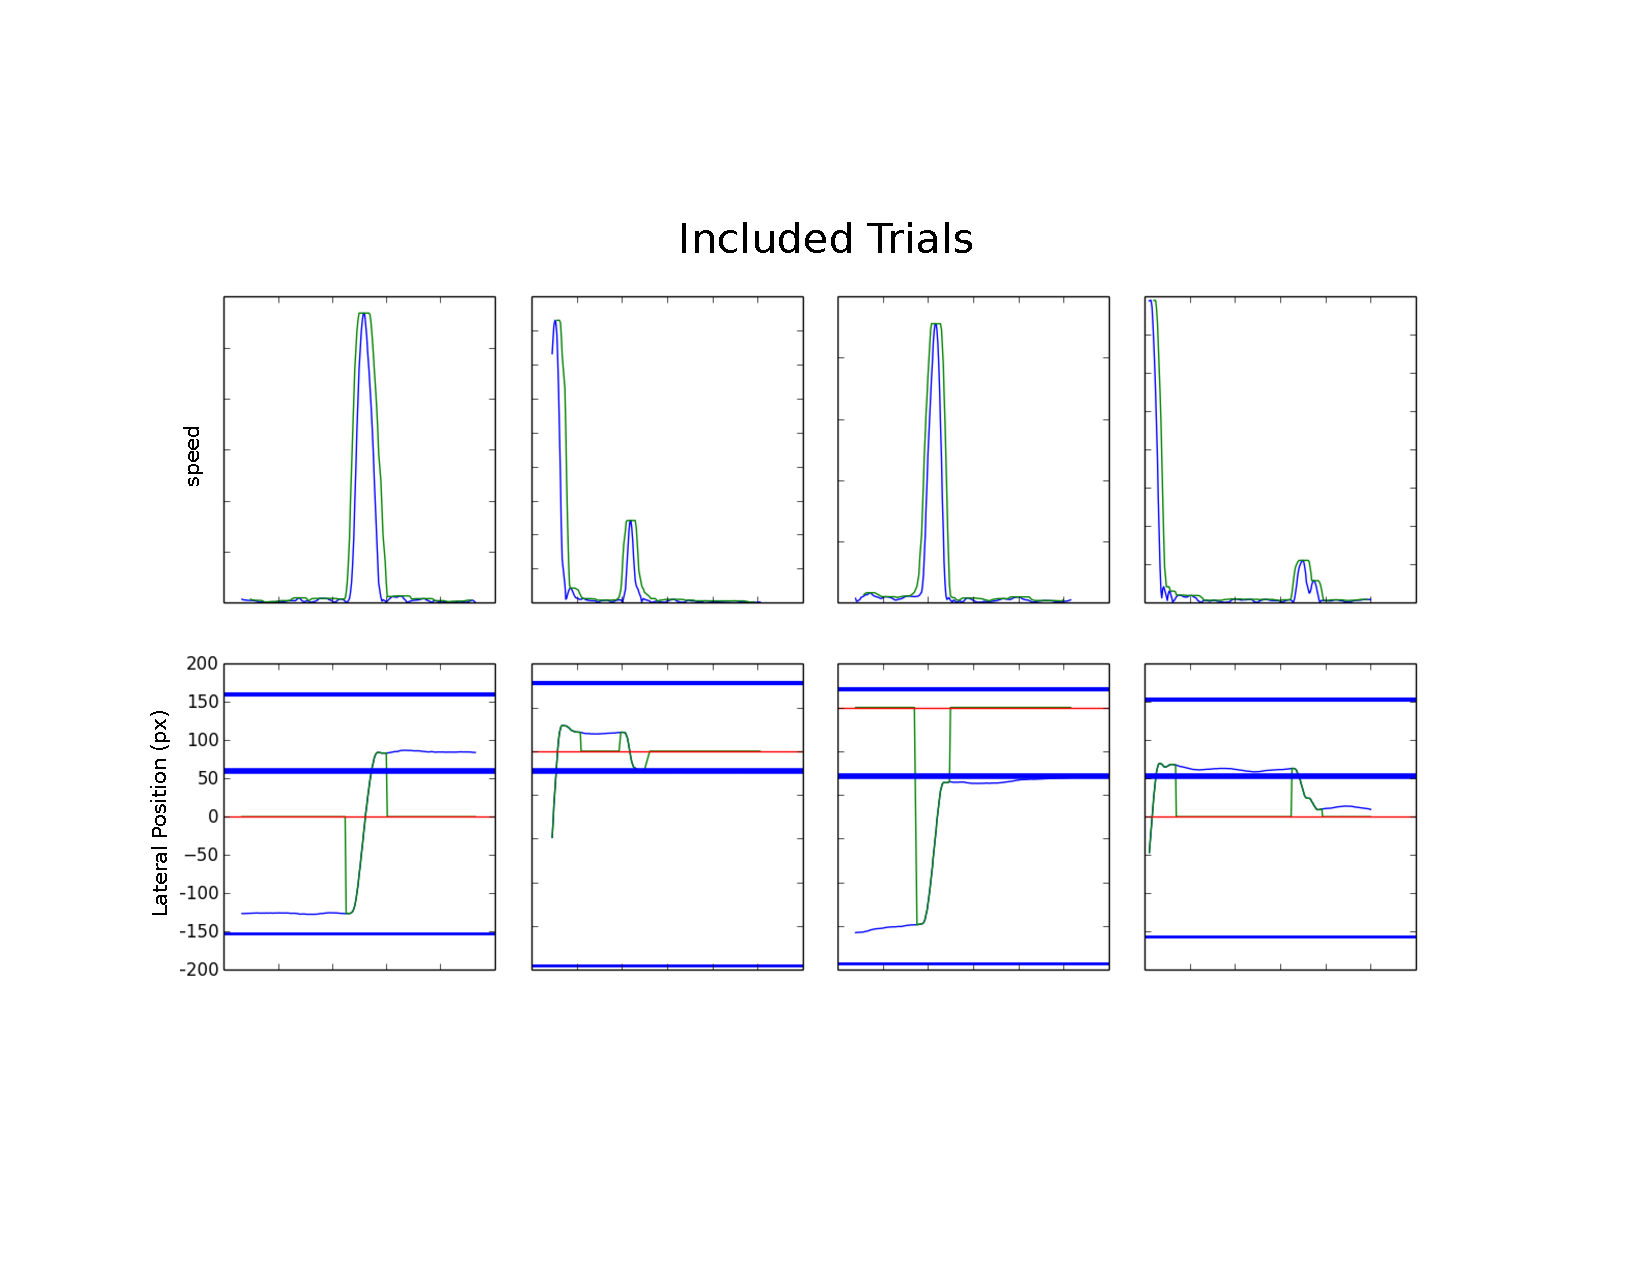
\includegraphics
	[height=1.1\textheight,width=1.1\textwidth,keepaspectratio]
	{appendix/accepted}
\end{frame}

\begin{frame}[noframenumbering]
	\frametitle{Rejected Trials}
	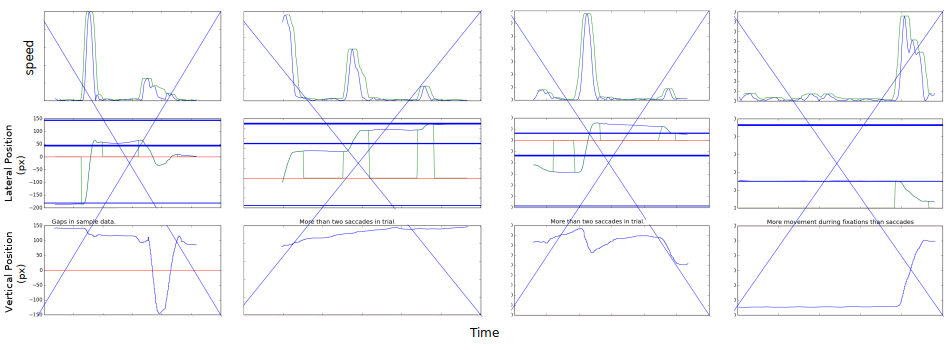
\includegraphics
	[height=1.1\textheight,width=1.1\textwidth,keepaspectratio]
	{appendix/rejected}
\end{frame}

\end{document}
